%% 
%% Copyright 2007, 2008, 2009 Elsevier Ltd
%% 
%% This file is part of the 'Elsarticle Bundle'.
%% ---------------------------------------------
%% 
%% It may be distributed under the conditions of the LaTeX Project Public
%% License, either version 1.2 of this license or (at your option) any
%% later version.  The latest version of this license is in
%%    http://www.latex-project.org/lppl.txt
%% and version 1.2 or later is part of all distributions of LaTeX
%% version 1999/12/01 or later.
%% 
%% The list of all files belonging to the 'Elsarticle Bundle' is
%% given in the file `manifest.txt'.
%% 
%% Template article for Elsevier's document class `elsarticle'
%% with numbered style bibliographic references
%% SP 2008/03/01

\documentclass[preprint,12pt]{elsarticle}%preprint,

%% Use the option review to obtain double line spacing
%% \documentclass[authoryear,preprint,review,12pt]{elsarticle}

%% Use the options 1p,twocolumn; 3p; 3p,twocolumn; 5p; or 5p,twocolumn
%% for a journal layout:
%% \documentclass[final,1p,times]{elsarticle}
%% \documentclass[final,1p,times,twocolumn]{elsarticle}
%% \documentclass[final,3p,times]{elsarticle}
%% \documentclass[final,3p,times,twocolumn]{elsarticle}
%% \documentclass[final,5p,times]{elsarticle}
%% \documentclass[final,5p,times,twocolumn]{elsarticle}

%% For including figures, graphicx.sty has been loaded in
%% elsarticle.cls. If you prefer to use the old commands
%% please give \usepackage{epsfig}

%% The amssymb package provides various useful mathematical symbols
\usepackage{amssymb}
\usepackage{booktabs}
\usepackage{amsmath}
\usepackage{algorithm}
\usepackage[noend]{algpseudocode}
\usepackage{algcompatible}
\usepackage{multirow}


%% The amsthm package provides extended theorem environments
%% \usepackage{amsthm}

%% The lineno packages adds line numbers. Start line numbering with
%% \begin{linenumbers}, end it with \end{linenumbers}. Or switch it on
%% for the whole article with \linenumbers.
%% \usepackage{lineno}
\journal{Computers \& Mathematics with Applications}
\bibliographystyle{elsarticle-num}
\begin{document}

\begin{frontmatter}

%% Title, authors and addresses

%% use the tnoteref command within \title for footnotes;
%% use the tnotetext command for theassociated footnote;
%% use the fnref command within \author or \address for footnotes;
%% use the fntext command for theassociated footnote;
%% use the corref command within \author for corresponding author footnotes;
%% use the cortext command for theassociated footnote;
%% and the form \ead[url] for the home page:
%% \title{Title\tnoteref{label1}}
%% \tnotetext[label1]{}
%% \author{Name\corref{cor1}\fnref{label2}}
%% \ead{email address}
%% \ead[url]{home page}
%% \fntext[label2]{}
%% \cortext[cor1]{}
%% \address{Address\fnref{label3}}
%% \fntext[label3]{}

\title{Optimised Cost Considering Huffman Code for
Biological Data Compression}

%% use optional labels to link authors explicitly to addresses:
%% \author[label1,label2]{}
%% \address[label1]{}
%% \address[label2]{}

%\author{}
\author[a,b]{Youcef Gheraibia\corref{cor1}}
\ead{Y.Gheraibia@hull.ac.uk}
\author[a]{Sohag Kabir\corref{cor2}}
\ead{s.kabir@hull.ac.uk}
\author[c]{Mohammad Kaykobad}
\author[d]{Abdelouahab Moussaoui}
\author[b]{Smaine Mazouzi}


\address[a]{Department of Computer Science, University of Hull, Hull HU6 7RX, UK}

\address[b]{Department of Computer Science, Badji Mokhtar-Annaba University, P.O. Box 12, 23000 Annaba, Algeria}


\address[c]{Department of Computer Science and Engineering, Bangladesh University of Engineering and Technology, Dhaka 1000, Bangladesh}

\address[d]{LRIA laboratory, Department of Computer Science, University of Setif, 19000, Algeria}



\cortext[cor1]{Corresponding author. Tel.: +44-7479-560709 ;}

\cortext[cor2]{Corresponding author. Tel.: +44-7405-024667 ; }



\begin{abstract}
%% Text of abstract
Classical Huffman code has widely been used to compress biological datasets. Though a considerable reduction of size of data is obtained by classical Huffman code, yet, more efficient encoding is possible by treating binary bits differently considering requirement of transmission time, energy consumption, and likewise. A number of techniques already modified Huffman code algorithm to  obtain optimal prefix-codes for unequal letter costs in order to reduce overall transmission cost (time). 
%In the recent year with the wide use of cloud and the distributed application in our life, the data transmission become more challenging over the years. 
In this paper we propose a new approach to improve compression performance of one such extension, cost considering approach (CCA),   %the data transmission technique by improving the representation of Huffman code with the use of a 
by applying genetic algorithm for optimal allocation of the codewords to the symbols. 
%The work in this research is consists of two steps. 
The approach start with generating a set of codewords for different input symbols based on their frequencies by considering cost (length) of 0 and 1 as $\alpha$ and $\beta$,~$\alpha < \beta$. This step ensures optimal cost encoding, however, compression performance is not higher than classical Huffman code. 
%The aim of the codes generation method is to minimise the number of ones on the generated codes, which minimise the cost of the transmission. 
%To improve compression performance, the second part of the approach uses genetic algorithm to find an optimal allocation of generated codes to different symbols. 
The idea is to sacrifice some cost to minimise total number of bits, hence, the genetic algorithm works by giving penalty on cost. The performance of the approach is evaluated by applying it to compress some standard biological datasets and comparing the result with the results produced by classical Huffman code and cost considering Huffman code.
% The case study of the approach is the biological data, which present a good application area to data compression with the huge growth of the biological data bases. 
%The results are very promising and we have compared with the standard cost considering Huffman code and the original Huffman code.
\end{abstract}

\begin{keyword}
Data Compression, Huffman code, Cost Considering Approach, Genetic algorithm, Biological data.
%% keywords here, in the form: keyword \sep keyword

%% PACS codes here, in the form: \PACS code \sep code

%% MSC codes here, in the form: \MSC code \sep code
%% or \MSC[2008] code \sep code (2000 is the default)

\end{keyword}

\end{frontmatter}

%% \linenumbers

%% main text
\section{Introduction}
\label{sec1}
In the recent years, application of battery-powered portable devices, e.g. laptop computers and mobile phones has increased significantly. Proper representation of digital data and their transmission efficiency has become a primary concern for digital community because it affects the performance, reliability, and the cost of computation in both portable and non-portable devices. CMOS technologies were developed in order to reduce the power consumption both in data processing and transmission. In order to increase transmission speed and reduce transmission cost, parallel data transmission methods are widely used. However, parallel transmission is limited to short distance communications, e.g. locally connected devices, internal buses. Ruling out the possible availability of parallel transmission links over long distance, we are left with its serial alternative only. If we attempt to transfer big files, e.g. DNA sequences, over a serial transmission link then it would take a significant amount of time. However, we cannot overlook this problem because at present parallel processing is widely used to increase throughput and in parallel processing architecture, processing units are usually distributed in different physical locations and task sharing is a must in such architecture.    
.
Data encoding techniques came into action to improve the data transmission efficiency over serial communication medium by compressing data before transmitting. Efficiency can be measured in terms of incurred cost, required storage space, consumed power, time spent and likewise. Data must be encoded to meet the purposes like: unambiguous retrieval of information, efficient storage, efficient transmission and etc. Let a message consist of sequences of characters taken from an alphabet $\Sigma$, where  $\delta_1,\delta_2,\delta_3\ldots,\delta_r$ are the elements that represent the characters in the source $\Sigma$. The length of $\delta_i$ represents its cost or transmission time, i.e., $cost\left(\delta_i\right)= length(\delta_i)$. A codeword $w_i$ is a string of characters in $\Sigma$, i.e., $w_i\in\Sigma^{+}$. If a codeword is $w_i=\delta_{i1},\delta_{i2},\ldots,\delta_{in}$, then the length or cost of the codeword is the sum of the lengths of its constituent elements:

\begin{equation}
\label{eqn1}
  \text{cost}\left(w_i\right)=\sum_{j=1}^{n}cost\left(\delta_{ij}\right)
\end{equation} 
  
If all the elements of a codeword has unit cost or length then the cost of the codeword is equivalent to the length of the codeword. However, it is not necessary for the elements in the codeword to have equal length or cost. For example, in Morse Code all the ASCII characters are encoded as sequence of dots ($\cdot$) and dashes ($-$) where a dash is three times longer than a dot in duration \cite{Redmond09}. However, the Morse code scheme suffers from the prefix problem \cite{Gr03}. Ignoring the prefix problem, Morse code results in a tremendous savings of bits over ASCII representation. Using Morse code, we can treat the binary bits differently; 0 as a dot and 1 as a dash. Even if we consider the voltage level to represent the binary digits then they are still different. Table \ref{table1} shows the logic level to represent binary digits in CMOS and TTL technologies. 

\begin{table}[h]
\renewcommand{\arraystretch}{1.5}
\caption{Example of binary logic level}
\label{table1}
\centering
\begin{tabular}{c c c c}
\hline
 \bfseries Technology  & 0 & 1&Notes\\
\hline
\bfseries CMOS & $0~V$ to $\frac{V_{DD}}{2}$&$\frac{V_{DD}}{2}$ to $V_{DD}$&$V_{DD}$= supply voltage\\
%\hline
\bfseries TTL & $0~V$ to $0.8~V$&$2~V$ to $V_{CC}$ &$V_{CC}$ is $4.75~V$ to $5.25~V$\\
%\hline
\hline
\end{tabular}
\end{table}

As the unequal letter cost problem is not new therefore it has been addressed by different researchers. The more general case where the costs of the letters as well as the probabilities of the words are arbitrarily specified was treated in \cite{Karp61}. A number of other researchers have focused on uniform sources and developed algorithm for the unequal letter costs encoding \cite{Gil95, Kar62,Varn71,AltMel80,perl1975}.  Let $p_1,p_2,\ldots,p_n$ be the probabilities with which the source symbols occur in a message and the codewords representing the source symbols are $w_1,w_2,\ldots,w_n$ then the cost of the code $W$ is:

\begin{equation}
C\left(W\right)=\sum_{i=1}^{n}cost\left(w_i\right).p_i 
\end{equation}
The aim of producing an optimal code with unequal letter cost is to find a codeword $W$ that consists of $n$ prefix code letters each with minimum cost $c_i$ that produces the overall minimum cost $C\left(W\right)$, given that costs $0<c_1\leq c_2 \leq c_2 \ldots \leq c_n$, and probabilities $p_1\geq p_2\geq \ldots\geq p_n>0$.

Huffman code\citep{Huff51} is an efficient data compression scheme that takes into account the probabilities at which different quantization levels are likely to occur and results in fewer data bits on the average. It is widely used to compress biological data, however, all the techniques use the classical form of the Huffman code where bits are treated equally. Out of many variations of the Huffman code where cost of bits are treated unequally, the most recent approach is described in \cite{Kab14}. This approach treated binary bit 0 as a dot $\left(\cdot\right)$ and 1 as a dash $\left(-\right)$ like Morse code and reduces the transmission cost (time) significantly. Like other variations of the cost considering Huffman code, the compression performance (in terms of number of bits require to encode a message) of this approach is not also better than classical Huffman code. In this paper, we have proposed a new optimised cost considering Huffman code based on the approach shown in \cite{Kab14}. This new approach optimised the number of bits require to encode biological datasets while treating the binary bits unequally. The codewords generated by the approach described in\cite{Kab14} only considers cost reduction but ignores bits reduction therefore number of total bits are considerably high. The proposed approach aims at reducing total number of bits   by applying a genetic algorithm. The algorithm works by giving penalty on cost to reduce number of bits, but also ensures that the overall cost is lower than classical Huffman code.  The efficiency of the method is evaluated by applying it to compress some standard biological datasets.         

The rest of the paper is organised as follows: Section~\ref{sec2} presents the background study of the issues in biological data processing and the Huffman code. The proposed approach is described in Section~\ref{sec3}. Experimental results and discussion are presented in Section~\ref{sec4} . Finally, concluding remarks are presented in Section~\ref{sec5}.



\section{Background}
\label{sec2}
\subsection{Issues in Biological Data Transmission}
The size of biological data including DNA sequences increase with an ever expanding rate and will be bigger and bigger in the future. These biological data are stored in biology databases. The exponential growth of these databases become a big problem to all biological data processing methods~\cite{Doug08}.
Different operations are applied to these data such as searching ~\cite{val10},e-mail attachment~\cite{chr09}, alignment ~\cite{che03}, and transmission on distributed computing platform~\cite{cha14}. Interestingly, biological data compression can play a key role in all sort of biological data processing. 

A recent deluge of interest in the development of new tools for biological data processing requires efficient methods for data compression. The main objective of data compression methods is minimising the number of bits in the data representation. 
In ~\cite{bra09}, authors proposed a new general data structure and data encoding approach for the efficient storage of genomic data. This method encodes only the differences between a genome sequence and a reference sequence. For encoding, the method uses different fixed-length encoding schemes such as Golomb\cite{Golomb96}, Elias codes\cite{Elias75} and variable codes such as Huffman codes. There are other methods based on the same idea of encoding only the difference between reference sequence and the target one. One such approach~\cite{chr09} uses Huffman code for encoding difference between sequences to sent it as an email attachment. The main limitation of this method is that it must send the reference sequence for at least once for each species, and usually this sequence is too big to be sent as an email attachment.
Wang and Zhang \cite{wan11} proposed a new scheme for referential compression of genomes based on the chromosome level. The algorithm searches for longest common subsequence between two sequences and then the differences between them are encoded using Huffman code.
All previous studies focus only on the differences and the relation between continuation of the sequence, and use existing encoding approaches to encode biological datasets without considering possible improvement of the encoding schemes.

%\subsection{Rationale of Unequal Bit Cost Considering Encoding Approaches}


\subsection{Huffman Codes}
In computer science and information theory, Huffman code is an entropy encoding algorithm used for lossless data compression. It takes into account the probabilities at which different symbols are likely to occur and results into fewer data bits on the average. 
%then assigns variable-length codes to different distinct symbols, and thus minimises the number of bits required to encode a message. 
For any given set of symbols and associated occurrence probabilities, there is an optimal encoding rule that minimises the number of bits needed to represent the source. Encoding symbols in predefined fixed length code, does not attain an optimum performance, because every character consumes equal number of bits irrespective to their degree of contribution to the whole data. Huffman code tackles this by generating variable length codes, given a probability usage frequency for a set of symbols. It generates prefix-code to facilitate unambiguous retrieval of information. A scheme of prefix code assigns codes to letters in $\Sigma$ to form codeword $w_i$ such that none of them is a prefix to another. For example, the codes $\left\{ 1,01,001,0001\right\}$ and $\left\{ 000,001,011,111\right\}$ are prefix-free, whereas the code $\left\{ 1,01,100\right\}$ is not, because 1 is a prefix in 100.

Applications of Huffman code are pervasive throughout
computer science. The algorithm to completely perform Huffman encoding and decoding is explained in \cite{Amst86}. It can be used effectively where there is a need for a compact code to represent a long series of a relatively small number of distinct bytes. For example, Table \ref{table2} shows 8 different ASCII characters, their frequencies, ASCII codes and the codewords generated for those symbols using Huffman code. It is seen from the table that the codeword to represent each character is compressed and the most frequent character gets the shortest code. In this example, the compression ratio obtained by Huffman code is 64.16\%.   

\begin{table}[h]
\renewcommand{\arraystretch}{1.3}
\caption{Example of application of Huffman Code to compress ASCII characters}
\label{table2}
\centering
\begin{tabular}{c c c c}
\hline
 Symbols & Frequency& ASCII Code &\begin{tabular}{@{}c@{}}Codewords using\\Huffman Code\end{tabular} \\
\hline
\bfseries A & 50&01000001&00\\
%\hline
\bfseries B & 35&01000010&101\\
%\hline
\bfseries C & 42&01000011&110\\
%\hline
\bfseries D & 22&01000100&1001\\
%\hline
\bfseries E & 65&01000101&01\\
%\hline
\bfseries F & 25&01000110&1111\\
%\hline
\bfseries G & 9&01000111&1000\\
%\hline
\bfseries H & 23&01001000&1110\\
\hline
\end{tabular}
\end{table}

There are many other variants of Huffman codes that compress source data to reduce data size and/or transmission cost. For example, Mannan and Kaykobad\cite{Kay03} introduced block technique in Huffman coding which overcomes the limitation of reading whole message prior to encoding. In the classical Huffman coding scheme, the letter costs are considered as equal. The unequal letter cost versions of Huffman codes scheme are proposed in \cite{Gol1996,Gol02,Gol2002,Gol12}.
In these versions, letters  of  the alphabet  are  treated  unequally. Recently, in \cite{Kab14} a method is proposed to show the effects of unequal bits cost on classical Huffman code. The idea of this method is to assign the most frequent symbol the minimum cost code and the least frequent symbol the maximum cost code, whereas classical Huffman code assigns most frequent symbol the minimum length code and the least frequent symbol the maximum length code. As a result, the approach in \cite{Kab14} produces an optimal prefix-codes for unequal letter cost, thus reduces the overall (transmission) cost of the encoded data. 

\section{The Proposed Approach}
\label{sec3}
%\subsection{}

A genome is a stretch of DNA that encodes  a polypeptide (protein)which is a set of amino acids bound together in a specific order. Each genomic sequence consists of nucleotides bound together, which are interpreted by the cellular machinery in groups of three, called triplets~\cite{Harvey00}. This is the main reason to divide the whole sequence in a set of triplet and give a code to each triplet. As each DNA sequence contains a combination of four nucleobases\textemdash guanine (G), adenine (A), thymine (T), and cytosine (C), therefore we will have $4^3=64$ possible triplets.  The first step in the optimised cost considering algorithm is cutting the genome sequence in triplets, then compute the frequency of each triplet in the whole sequence. This table of frequencies are used by the cost considering Huffman code to generate minimal cost code for each triplet (frequency). Finally, these codes with frequencies are used by the optimised cost considering algorithm to generate the optimal allocation with a given  penalty on cost. The whole process is shown in Fig.1.%\ref{Fig1}.

\begin{figure}[t]
\begin{center}
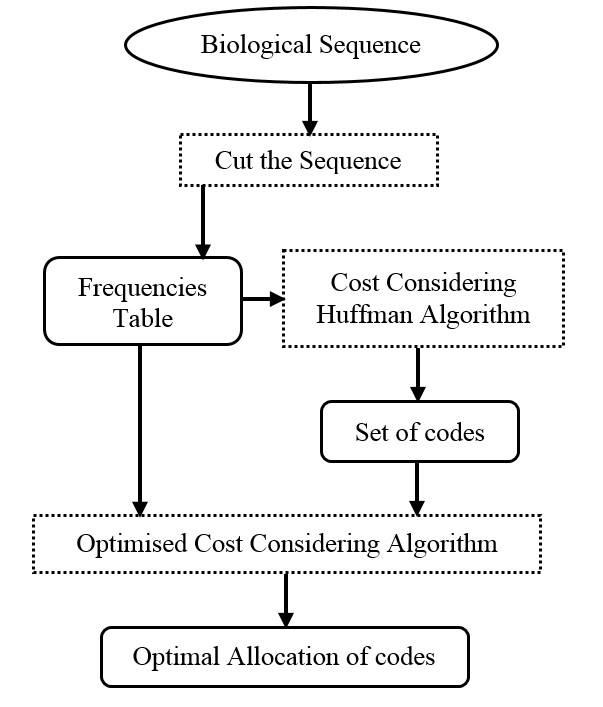
\includegraphics[scale=0.4]{Images/Drawing3_1.jpg}
\caption{The proposed scheme}
\end{center}
\label{Fig1}
\end{figure}

\subsection{Cost Considering Approach of Huffman code}
The classical Huffman algorithm aims at reducing total number of bits and it constructs a tree in a bottom up fashion. It is shown in \cite{golin98} that if the costs of letters are considered unequal then the straightforward bottom up greedy approach does not work. Authors in \cite{Kab14} uses a top down approach to build a binary tree considering unequal letter cost of bits. They considered cost (length) of 0 and 1 as integer constants $\alpha$ and $\beta$,   $\alpha < \beta$. Using the analogy of Morse code's `$\cdot$' and `$-$', the value of $\alpha$ and $\beta$ is set as 1 and 3 respectively. The complete algorithm to obtain an optimal prefix-free code for unequal letter cost is shown below (algorithm 1). The input to the algorithm are the distinct triplets contained in the genome sequence to be encoded and their frequencies. The process of creating the binary tree starts with a single node (root node) and it is initialised with cost 0.  After that, two child (leaf) nodes are created for the root node, i.e., level of the tree is increased by one. Cost of the left child is calculated as the summation of the cost of its parent node and the length of the left arc, and cost of the right child is calculated as the summation of the cost of its parent node and the length of the right arc. Length of left and right arcs are actually the cost (length) of 0 ($\alpha$) and 1 ($\beta$) respectively. The next step is to take a child node with least cost and create two child nodes for it and make it a parent node. In this way, in every iteration the child node with least cost becomes a parent node with two new child nodes. Creation of new child nodes is stopped when total number of child nodes become equal to the number of distinct triplets needed to be encoded. 

\begin{algorithm}[!btph]
\caption{Cost Considering Algorithm (CCA)}
\label{alg1}

\begin{algorithmic}[1]
\REQUIRE Distinct symbols contained in the message to be encoded and their frequencies 
\ENSURE Non-uniform\ /\ variable\ letter\ cost\ i.e,\ Cost-considering\ balanced\ tree

\FOR{each distinct symbol $i$} 
\STATE $ Enqueue\left(max\_Q , frequency~[~i~]\right)$
\ENDFOR
\STATE create a root node
\STATE $cost~[~root~]\leftarrow 0$
\STATE $Enqueue\left(min\_Q , cost~[~root~]\right)$
\STATE Define costs of the left and right child of the binary tree
\REPEAT 
\STATE $cost\_of\_parent\_node\leftarrow Dequeue\left(min\_Q\right)$
\STATE create $left$ and $right$ child for this node
\STATE $cost~[~left\_child~]\leftarrow cost\_of\_parent\_node+left\_child\_cost$
\STATE $Enqueue\left(min\_Q , cost~[~left\_child~]\right)$
\STATE $cost~[~right\_child~]\leftarrow cost\_of\_parent\_node+right\_child\_cost$
\STATE $Enqueue\left(min\_Q , cost~[~right\_child~]\right)$
\STATE Mark parent node as explored
\UNTIL{$2\left(n-1\right)$ nodes are created}
\WHILE{$min\_Q\neq\emptyset$} 
\STATE $leaf\_node\leftarrow Dequeue\left(min\_Q\right)$
\STATE $frequency[leaf\_node]\leftarrow Dequeue\left(max\_Q\right)$
\ENDWHILE
\FOR{each parent node $j$} 
\STATE $frequency~[~j~]\leftarrow frequency~[~left\_child~]+frequency~[~right\_child~]$
\ENDFOR
\REPEAT
\IF{conflict between nodes} 
\STATE resolve conflict by swapping conflicted nodes
\STATE calculate and reassign cost of all affected nodes
\STATE calculate and reassign frequency of all affected nodes 
\ENDIF
\UNTIL{all conflicts are resolved }
%\algstore{myalg}
\end{algorithmic}
\end{algorithm}

Now the tree $T$ is constructed and the cost of the tree actually depends on how the frequencies are assigned to the leaf nodes. The overall cost will be minimised if the leaves with highest cost always have smaller or equal weight (frequency). To fulfil this condition the leaves of the $T$ are enumerated in non-decreasing order of their cost, i.e., $cost(l_1)\leq cost(l_2)\leq \ldots \leq cost(l_n),$ and that $f_1 \geq f_2 \geq \ldots\geq f_n$, where $l_i$ and $f_i$ are leaf nodes and frequencies of distinct triplets respectively $for~ i=1,2,\ldots n$ . The frequency or weight of parent nodes are calculated as the sum of the frequencies of its child nodes, and it continues upwards until the root node is reached. After that, the algorithm checks for any possible conflicts between all pair of nodes. Two nodes are considered as conflicted if the node with a higher cost has higher frequency violating the above condition, i.e., if $cost(l_i)> cost(l_j)~and~f(l_i)>f(l_j)$, then there remains a conflict.  If there remains a conflict between nodes, then it is resolved by swapping the nodes and recalculating the cost of the tree downward and frequency of the nodes upward.  When all the conflicts if existed are resolved then the algorithm generates codes for each of the distinct triplets.   

\subsection{Optimisation of the Codes}
\subsubsection{Problem formulation}
The problem of finding the best allocation of codes to each triplet can be   modelled as an assignment problems, the problem is formulated as follows :\\\\
\textbf{Definition:} Given a set of codes $C=\left\{C_{1},C_{2}...C_{n}\right\}$, and a set of frequencies $F=\left\{F_{1},F_{2}...F_{n}\right\}$. For each code we have the length of the code $|C_{i}|$ (number of bits) and the cost of the code $S_{C_{i}}$, the objective is to assign to each frequency a code in order to minimise the total number of bits, while respecting the initially assigned total cost $S_{t}$ with a given penalty $\lambda\rightarrow [0,1]$. This penalty coefficient represents the allowed amount of cost that can be sacrificed to optimise the total number of bits.    
\\
The Objective Function is to: 

\begin{equation}
Minimise \sum (|C_{i}| \times F_{j})
\end{equation}
while :
\begin{equation}
\sum (|S_{C_{i}}| \times F_{j}) \leqslant (\lambda+1) S_{t} 
\end{equation}

\subsubsection{Basic Genetic Algorithm}
Genetic Algorithm (GA) is a bio-inspired meta-heuristic algorithm developed by \cite{gen1}. GA is a stochastic optimisation algorithm imitate the natural evolution process of genomes. GA started by generating an initial population of random feasible solutions. The optimisation process of GA takes the initial population and generates a new population based on it.  The process can be described as follow:\\ 
Firstly, select two or more solutions from the current population by using one of the well-known selection techniques \cite{bli95}. These selected solutions will be considered as  parents. The second operation of the genetic algorithm is the crossover, which takes these parents as inputs to generate other new solutions considered as children. The third operation of the genetic algorithm is the mutation which ensures a good diversification in the search process. The new solutions can be mutated according to a given mutation probability. The mutation operation changes the value of one or more positions in the solution. The quality of each solution is verified by the fitness function which controls the evolution of the GA population by deletion of the worst solutions and insertion of the good solutions among  parents and sons. This processes is repeated until the stopped criteria is reached which can be the number of generation or if the population is stabilised.

\subsubsection{Optimised cost considering algorithm}
The main objective of the optimised cost considering algorithm (OCCA)is to apply GA to find an optimal allocation of the codewords to each triplets to reduce the total number of bits. In GA, the encoding of the solution into a chromosome is one of the most important issues in obtaining good optimisation results. The OCCA uses two fixed length arrays of size ``64" which is the number of combination for all nucleotides. The first array contains the frequencies of each triplets and the second array contains the cost of the codewords assigned to each triplets. Our genetic algorithm utilises the two arrays and uses the index of each entries in the allocation process.

The genetic algorithm is a stochastic algorithm based on random evolution process. The algorithm 2 describes the outline of the OCCA.   Generally the initial population is generated in a random affectation of codes to different triplets. In the OCCA algorithm, the population contain firstly the affectation given by the CCA. The rest of the population are randomly generated, all these generated solutions must satisfy the initial cost constraints, which is the cost ($S_t$) of the solution produced by CCA  and previously added to the population with a give penalty (step 1). 

The evolution of the population is the key of the genetic optimisation algorithm. During each generation the process start with the selection of a part (set of solutions) of the population to bread a new generation. In the literature many selection methods have been proposed to guide the population evolution \cite{bli95}. The different methods for selecting a part (set of solutions) of the population vary from a random selection method to heuristic based selection method. We have chosen to select randomly the part of the population to be processed as the heuristic methods are very time-consuming (step 3).
After that the operations of genetic algorithm is applied on the initial population to generate a new generation of the population (see Fig.2). Firstly the crossover operation is applied to these two selected solutions (considered as parents) to generate two new solutions (considered as children)(step 4). In the literature many crossover techniques have been used in genetic algorithm \cite{osa14}, such as one-point crossover which divides the chromosomes into two fragments and recombines the second fragments with the other chromosome's second fragment. The two-point crossover divides the chromosomes into three fragments and recombines the middle fragment with  the middle fragment of the other chromosome. There are many other crossover techniques to allow a good convergence of the algorithm. In our case, we have used the two point crossover with two parameters, the first parameter $p_{c}$ is a random value in [0,63], which represents the first cut point and the second parameter $p_{m}$ is also a random value in [0,63], which represents the number of positions to be crossed. These two random parameters are to ensure a good diversification on the whole search space (step 4).

\begin{figure}[h]
\begin{center}
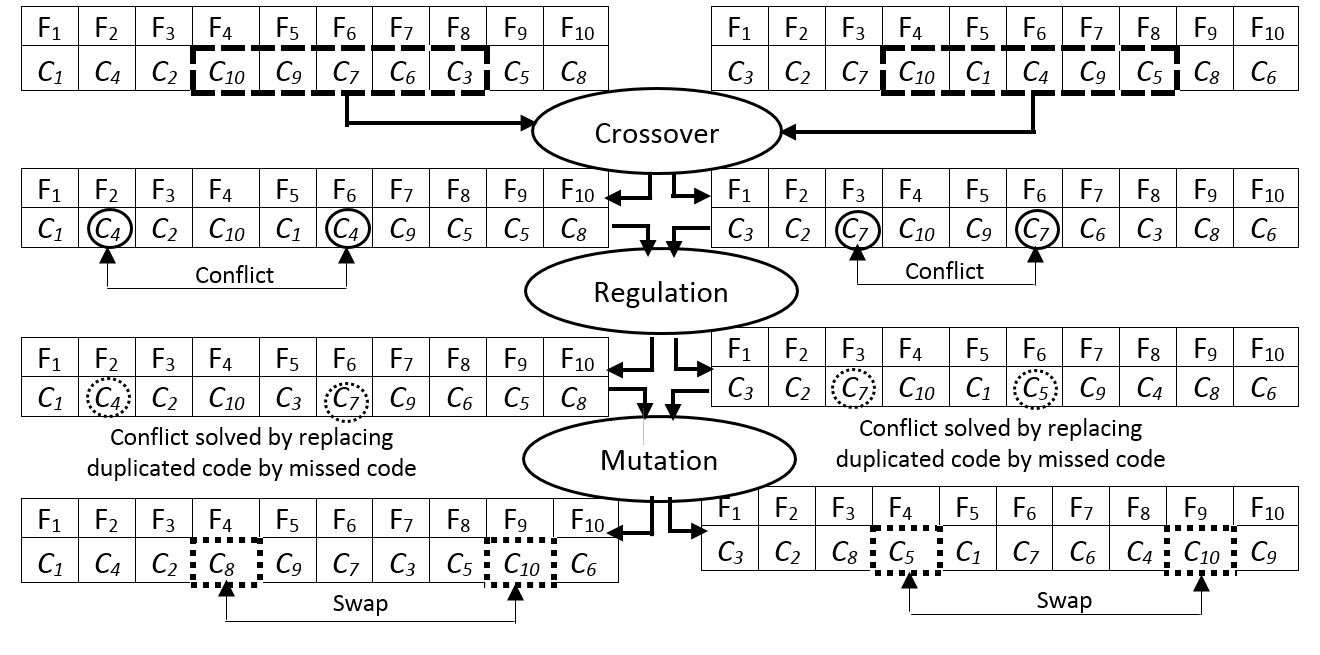
\includegraphics[scale=0.5]{Images/Drawing2.jpg}
\caption{Operations of genetic algorithm}
\end{center}
\label{Fig3}
\end{figure}

\begin{figure}[!thpb]
\begin{center}
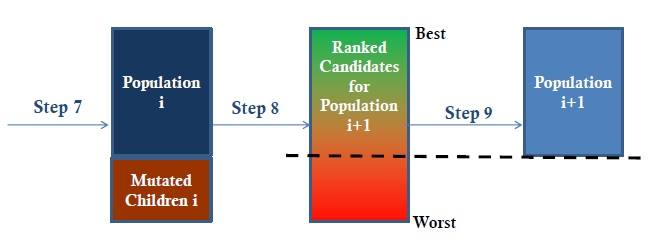
\includegraphics[scale=0.55]{Images/Drawing_1.jpg}
\caption{Population update for genetic algorithm}
\end{center}
\label{Fig2}
\end{figure}

\begin{algorithm}[!thpb]
\caption{Optimised Cost Considering Algorithm (OCCA)}
\begin{algorithmic}[1]
\State Population initialization (P).
\REPEAT  
\State Select two solutions $S_{1},S_{2}$ form P.
\State Crossover $S_{1},S_{2}$ to generate $S_{11},S_{21}$ (Children).
\State Mutate $S_{11},S_{21}$.
\State Validate children with cost constraint (equation 4). 
\State Add children to population
\State Rank the population by fitness
\State Remove worst candidates until population limit
\UNTIL{Max number of generation not achieved} 
\EndWhile
\State Display the best solution from the population P;
\end{algorithmic}
\end{algorithm}


After the crossover operation, the newly generated children may contain conflict, for example, a single code is allocated to two different frequencies in the solution. To overcome such a conflict, a regulation operation is performed to refine the solution to ensure the correctness of the solution (see Fig.2).
 Secondly these two new solutions are mutated according to a predefined probability $\gamma$, the best value of the mutation rate is very problem specific (step 5). In our case, the value of $\gamma$ is fixed to $0.2$ to explorer a few positions in the solution. The mutation operator is used to maintain genetic diversity from one generation of the population of genetic algorithm to the next. In our case, we have used the mutation as a random swap mutation operator (see Fig.3).  Each newly generated solution must satisfy the cost constraint. The next step is to add these two new solutions (children) to the current population (step 7) (see Fig. 3). Finally, the new population are ranked by fitness (step 8), and the worst solutions are deleted until the initial size of the population is obtained  (step 9). The whole processes are repeated until the maximum number of operation is performed (step 10). 


\section{Results And Discussion}
\label{sec4}
The effectiveness of the approach has been evaluated with different real genomic biological data, these genomes were downloaded from a recent version of The National Center for Biotechnology Information (NCBI) available on $(http://www.ncbi.nlm.nih.gov)$ \cite{pruitt2009ncbi}. We focused on the sequences alone, ignoring any header and any other exogenous information. In table 3, the different data sets are described with the size  of each of them in megabytes (MB) and the references on the biological data bank.

\begin{table}[!thpb]

\small
\label{table3}
\caption{Datasets description}
%\begin{center}
\centering
\begin{tabular}{c  c  c c}
\toprule
$\textbf{Data sets}$ &$\textbf{Name}$ &	$\textbf{Size (MB)}$ &	$\textbf{Reference}$ \\\hline
Genome 1& Mycobacterium smegmatis &  6.66 & CP009496  \\\hline

Genome 2& Amycolatopsis benzoatilytica & 8.30 & NZ\_KB912942 \\\hline

\multirow{2}{*}{Genome 3}&Mycobacterium rhodesiae& \multirow{2}{*}{6.11} & \multirow{2} {*}{CP003169}\\ 
&NBB3& &\\
\hline

\multirow{2}{*}{Genome 4 }&Streptomyces bottropensis& \multirow{2}{*}{8.54} &
\multirow{2}{*}{NZ\_KB911581} \\ 
& ATCC 25435 \\
\hline
    
\multirow{2}{*}{Genome 5}&Mycobacterium smegmatis& \multirow{2}{*}{ 6.66} &\multirow{2}{*}{CP009494             } \\ 
&str. MC2 155 \\
\hline

\multirow{2}{*}{Genome 6}&Mycobacterium smegmatis& \multirow{2}{*}{6.76} &\multirow{2}{*}{NZ\_KI421511}\\   &MKD8& &\\
\hline
    
Genome 7& Bradyrhizobium WSM471&  7.42 &NZ\_CM001442\\\hline

\multirow{2}{*}{Genome 8}&Amycolatopsis thermoflava&  \multirow{2}{*}{8.27} &\multirow{2}{*}{NZ\_CM001442}\\   &N1165 & \\
\hline

\multirow{2}{*}{Genome 9}&Bacillus thuringiensis&   \multirow{2}{*}{5.74} &\multirow{2}{*}{ NZ\_CM000747 }\\    &Bt407&\\
\hline    

\multirow{2}{*}{Genome 10}&Bacillus thuringiensis& \multirow{2}{*}{6.03} &\multirow{2}{*}{ NZ\_CM000748}\\    &serovar thuringiensis& \\
\hline
    
\multirow{2}{*}{Genome 11}&Pseudomonas aeruginosa& \multirow{2}{*}{6.48} &\multirow{2}{*}{NZ\_AFXI01000001}\\    &9BR&\\
\hline
    
\multirow{2}{*}{Genome 12}&Bacillus thuringiensis&  \multirow{2}{*}{5.97} &\multirow{2}{*}{ NZ\_CM000753}\\    &serovar berliner ATCC &\\
\hline
    
\multirow{2}{*}{Genome 13}&Bacillus thuringiensis& \multirow{2}{*}{5.75} &\multirow{2}{*}{ NZ\_CM000750 }\\    &serovar pakistani&\\
\hline
    
\multirow{2}{*}{Genome 14}&Pseudomonas aeruginosa& \multirow{2}{*}{6.28} &\multirow{2}{*}{CP006982}\\    &LES400&\\
\hline

\multirow{2}{*}{Genome 15}& Mus musculus & \multirow{2}{*}{25.58} &\multirow{2}{*}{GL456087}\\  &chromosome 1&\\
\hline

\multirow{2}{*}{Genome 16}& Danio rerio & \multirow{2}{*}{56.14} &\multirow{2}{*}{CM002885}\\ & chromosome 1 &\\
\hline
\multirow{2}{*}{Genome 17}&Homo sapiens & \multirow{2}{*}{76.64 } &\multirow{2}{*}{  CM000680  }\\    & chromosome 18 &\\
\hline
\multirow{2}{*}{Genome 18}&Homo sapiens & \multirow{2}{*}{99.94} &\multirow{2}{*}{CM000684   }\\ & chromosome 22&\\
\hline
%\bottomrule
\end{tabular}
%\end{center}
\end{table} 

\begin{table}[h]
\renewcommand{\arraystretch}{1.1}
\small
\label{table4}
\caption{Comparison of performance among classical Huffman code, CCA, and OCCA without penalty}
%\begin{center}

\begin{tabular}{c  c c  c c  c c}
\hline
 & \multicolumn{2}{c}{Huffman Algorithm} & \multicolumn{2}{c}{CCA }& \multicolumn{2}{c}{OCCA \textit{($\lambda$=0)}}\\\hline
$\textbf{Data sets}$ & $\textbf{Cost}$	& $\textbf{Size(MB)}$ &	$\textbf{Cost}$&	$\textbf{Size(MB)}$&$\textbf{Cost}$&	$\textbf{Size(MB)}$
\\\hline
Genome 1& 76787151  &	4.44	&67416213   & 4.92	& 67416213 & 4.82 \\\hline
Genome 2& 100425402 &  	5.81	& 88430665	& 6.51	& 88430665&  6.35 \\\hline
Genome 3& 75940155  &	4.39    &66745619	& 4.87&	66745619 & 4.79 \\\hline
Genome 4& 103552729 &	5.96    &90821835&	6.69 &	90821835  & 6.47\\\hline
Genome 5& 82234926  &	4.74	&71963876	& 5.27 &	71963876 &5.17 \\\hline
Genome 6& 83454842  &   4.81	&73038795	& 5.34	&73038795 & 5.24\\\hline
Genome 7& 92539488  &	5.36    &81416359   &5.93	&81416359 & 5.85\\\hline
Genome 8& 99613856  & 	5.74	&87102639   &6.41	&87102639&	6.30 \\\hline
Genome 9& 71876739  &	4.15    &62998800  &4.58 &	62998800 &	4.49 \\\hline
Genome 10& 75324432 & 	4.36	&66084958  &4.81	&66084958&	4.73 \\\hline
Genome 11& 80766360 &	4.66    &70620666  &5.41&	70620666&	5.04 \\\hline
Genome 12& 74560825 &	4.31    &65359604  &4.75	&65359604&	4.67\\\hline
Genome 13& 71562941 & 	4.14	&62758225  &4.56	&	62758225 &	4.50\\\hline
Genome 14& 78261299 & 	4.51    &68354090  &4.8&	68354090& 4.89  \\\hline
Genome 15& 324439242& 	18.77    &286008420 & 20.66	 &	286008420 &	19.94 \\\hline
Genome 16& 703734840&  40.77    &618859291 & 45.08  &	618859291 &	43.18 \\\hline
Genome 17& 901032667&  52.08    &791840455 &	57.36 &	791840455 &	55.12 \\\hline
Genome 18& 983434816&  56.98    &867299889 &	62.42 &	867299889 & 60.70 \\\hline

%\bottomrule
\end{tabular}
%\end{center}
\end{table}

\begin{figure}[h]
\begin{center}
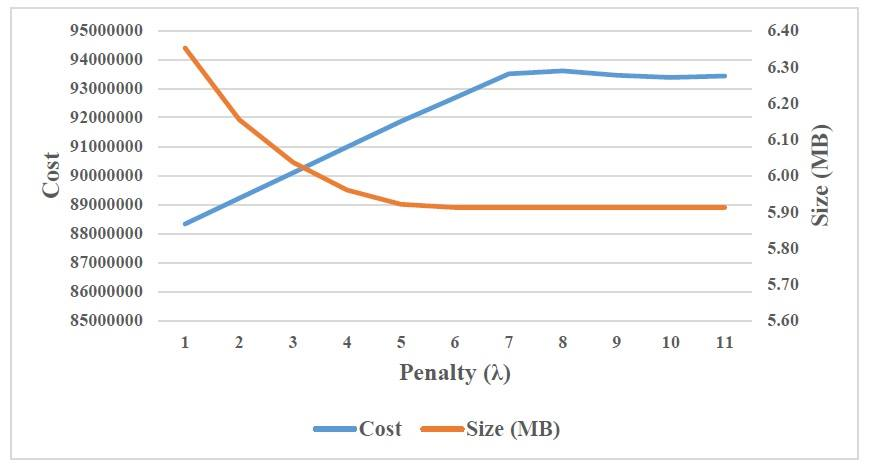
\includegraphics[scale=0.45]{Images/drawing4_1.jpg}
\caption{Convergence of OCCA for \textit{Genome 2}}
\end{center}
\label{Fig5}
\end{figure}


\begin{table}[tpbh]
\small
\renewcommand{\arraystretch}{1.1}
\caption{Effects of  the penalty on the compression performance of the OCCA}
%\begin{center}
\centering
\begin{tabular}{c c c c c }
\toprule
$\textbf{Data sets}$ & $\textbf{Cost}$	& $\textbf{Size(MB)}$ &		\textbf{$\lambda (\%)$} &		\textbf{Compression ratio $\%$} \\\hline
Genome 1 &	 70760174 &4.50& 4\% & 32.72\%\\\hline
Genome 2 &	92010490& 5.91 & 5\%& 28.79\%\\\hline
Genome 3&	69421783& 4.47 &3\%& 26.84\%\\\hline
Genome 4&	96294638& 5.99 & 5\%& 29.85\%\\\hline
Genome 5&	74855668 &4.81& 5\%& 27.77\%\\\hline
Genome 6&	76738330& 4.86  &4\%& 28.10\%\\\hline
Genome 7&	84667949 &5.47& 3\%& 26.28\%\\\hline
Genome 8&	92416243 &5.76& 5\%& 30.35\%\\\hline
Genome 9&	66145783&4.21 & 4\%& 26.65\%\\\hline
Genome 10&	68751359& 4.44 &3\%& 26.63\%\\\hline
Genome 11&	72737300 &4.79& 2\%&26.08\%\\\hline
Genome 12&	67981988 & 4.38&3\%& 26.63\%\\\hline
Genome 13&	65896779& 4.18 &4\%& 27.30\%\\\hline
Genome 14&	71762305 &4.55 &4\%&27.54\% \\\hline
Genome 15&297188002 &19.31 & 3\%& 24.51\%\\\hline
Genome 16&643785655 & 41.68 & 3\%& 25.75\% \\\hline
Genome 17&823506882 & 53.05 & 3\%& 30.78\%\\\hline
Genome 18&901515198 &58.99 & 3\%& 40.97\%\\
\bottomrule
\end{tabular}
%\end{center}
\label{table5}
\end{table}


Table~\ref{table4} presents the results obtained by the classical Huffman code, the cost considering algorithm (CCA) and the optimised cost considering algorithm (OCCA) without penalty on cost. The results show that the number of bits required by the classical Huffman algorithm to encode genomic data is the minimum among the other algorithms but the cost is  maximum. The cost considering algorithm improves the representation of the generated codes in terms of cost but the number of bits. However, still it compresses the data by $37.54\%$ in the best case, $16.51\%$ in the worst case, and $22.08\%$ on an average. In terms of cost, in the best case the CCA improves cost over classical Huffman code by $12.66\%$, in the worst case by $11.80\%$, and on an average by $12.24\%$.  The optimised cost considering algorithm tries to find the best allocation of codes to frequencies by giving penalty on cost. The outcome of this process is a fall in the total number of bits and a rise in the total cost. However, the cost is always lower than the cost incurred by the classical Huffman algorithm.  At first, the OCCA optimises number of bits without applying any penalty on the cost (see table 4). Afterwards, it continues giving penalty ranging from 1\% to 10\% on the cost  until a balance is found between total cost and bits. Fig. 4 shows the convergence of the OCCA for minimising number of bits for genome 2 according to the cost constraint. For each genome, a maximum amount of effective penalty is identified, after this maximum value, increasing the penalty is not helping any more to reduce number of bits, i.e., number of bits reach to minimum and cost to maximum.  The table \ref{table5} presents the best founded number of bits for different datasets with different effective penalty. As seen in the table, the OCCA improves the compression ratio from $37.54\%$ to $40.97\%$ in the best case, from $16.51\%$ to $24.51\%$ in the worst case, and from $22.08\%$ to $28.53\%$ in the average case. This is evident from the table 5 that this improvement is obtained without increasing the cost significantly.    %are in-useful (See figure 3), the number of bits achieve the minimum number but the cost stop decreasing (point 1 in figure 3) and this number of bits stabilized while the cost still increasing until it stabilized also (point 2 figure 3), after this point the cost and number of bits are stabilized.

\section{Conclusion}
\label{sec5}
In this paper, we have discussed how the cost considering  algorithm (CCA) of Huffman code~\cite{Kab14} can be used to efficiently compress  biological datasets to facilitate efficient data transmission. The advantage of CCA is that it significantly improves (transmission) cost over classical Huffman code given that the cost of bits are different, however, it takes more bits than the classical Huffman code to encode data. In this paper, we identified genetic algorithm as a potential method to optimise the total number of bits in the CCA. The proposed optimised cost considering approach (OCCA) starts its operation by generating a set of optimal prefix-free codewords for a set of distinct input symbols by applying CCA which treats binary bits unequally. 

 After that, the approach utilises genetic algorithm to find an optimal allocation of generated codewords to different symbols to reduce the total number of bits require to encode the dataset. In this allocation process the OCCA gives penalty on the cost to improve the compression performance.
 
The proposed approach is applied to biological genomic datasets and a performance comparison is made with the standard Huffman code and the cost considering algorithm of the Huffman code. The results show that the proposed approach improves the compression performance of the CCA significantly without affecting the cost notably. In future, we hope to extend this work by reducing number of switching activity between the codewords to further reduce the cost of transmission.
%is more robust and efficient compared to other competing algorithms because its penalty based optimisation strategy to search the best allocation of codes to different frequencies.

%% The Appendices part is started with the command \appendix;
%% appendix sections are then done as normal sections
%% \appendix
%% \section{}
%% \label{}
%% If you have bibdatabase file and want bibtex to generate the
%% bibitems, please use
%%
%%  \bibliographystyle{elsarticle-num} 
%%  \bibliography{<your bibdatabase>}

%% else use the following coding to input the bibitems directly in the
%% TeX file.

%\begin{thebibliography}{00}

%% \bibitem{label}
%% Text of bibliographic item

%\bibitem{}

%\end{thebibliography}

\section*{References}
\bibliography{mybibfile}
\end{document}
\endinput
%%
%% End of file `elsarticle-template-num.tex'.
